\documentclass[1p]{elsarticle_modified}
%\bibliographystyle{elsarticle-num}

%\usepackage[colorlinks]{hyperref}
%\usepackage{abbrmath_seonhwa} %\Abb, \Ascr, \Acal ,\Abf, \Afrak
\usepackage{amsfonts}
\usepackage{amssymb}
\usepackage{amsmath}
\usepackage{amsthm}
\usepackage{scalefnt}
\usepackage{amsbsy}
\usepackage{kotex}
\usepackage{caption}
\usepackage{subfig}
\usepackage{color}
\usepackage{graphicx}
\usepackage{xcolor} %% white, black, red, green, blue, cyan, magenta, yellow
\usepackage{float}
\usepackage{setspace}
\usepackage{hyperref}

\usepackage{tikz}
\usetikzlibrary{arrows}

\usepackage{multirow}
\usepackage{array} % fixed length table
\usepackage{hhline}

%%%%%%%%%%%%%%%%%%%%%
\makeatletter
\renewcommand*\env@matrix[1][\arraystretch]{%
	\edef\arraystretch{#1}%
	\hskip -\arraycolsep
	\let\@ifnextchar\new@ifnextchar
	\array{*\c@MaxMatrixCols c}}
\makeatother %https://tex.stackexchange.com/questions/14071/how-can-i-increase-the-line-spacing-in-a-matrix
%%%%%%%%%%%%%%%

\usepackage[normalem]{ulem}

\newcommand{\msout}[1]{\ifmmode\text{\sout{\ensuremath{#1}}}\else\sout{#1}\fi}
%SOURCE: \msout is \stkout macro in https://tex.stackexchange.com/questions/20609/strikeout-in-math-mode

\newcommand{\cancel}[1]{
	\ifmmode
	{\color{red}\msout{#1}}
	\else
	{\color{red}\sout{#1}}
	\fi
}

\newcommand{\add}[1]{
	{\color{blue}\uwave{#1}}
}

\newcommand{\replace}[2]{
	\ifmmode
	{\color{red}\msout{#1}}{\color{blue}\uwave{#2}}
	\else
	{\color{red}\sout{#1}}{\color{blue}\uwave{#2}}
	\fi
}

\newcommand{\Sol}{\mathcal{S}} %segment
\newcommand{\D}{D} %diagram
\newcommand{\A}{\mathcal{A}} %arc


%%%%%%%%%%%%%%%%%%%%%%%%%%%%%5 test

\def\sl{\operatorname{\textup{SL}}(2,\Cbb)}
\def\psl{\operatorname{\textup{PSL}}(2,\Cbb)}
\def\quan{\mkern 1mu \triangleright \mkern 1mu}

\theoremstyle{definition}
\newtheorem{thm}{Theorem}[section]
\newtheorem{prop}[thm]{Proposition}
\newtheorem{lem}[thm]{Lemma}
\newtheorem{ques}[thm]{Question}
\newtheorem{cor}[thm]{Corollary}
\newtheorem{defn}[thm]{Definition}
\newtheorem{exam}[thm]{Example}
\newtheorem{rmk}[thm]{Remark}
\newtheorem{alg}[thm]{Algorithm}

\newcommand{\I}{\sqrt{-1}}
\begin{document}

%\begin{frontmatter}
%
%\title{Boundary parabolic representations of knots up to 8 crossings}
%
%%% Group authors per affiliation:
%\author{Yunhi Cho} 
%\address{Department of Mathematics, University of Seoul, Seoul, Korea}
%\ead{yhcho@uos.ac.kr}
%
%
%\author{Seonhwa Kim} %\fnref{s_kim}}
%\address{Center for Geometry and Physics, Institute for Basic Science, Pohang, 37673, Korea}
%\ead{ryeona17@ibs.re.kr}
%
%\author{Hyuk Kim}
%\address{Department of Mathematical Sciences, Seoul National University, Seoul 08826, Korea}
%\ead{hyukkim@snu.ac.kr}
%
%\author{Seokbeom Yoon}
%\address{Department of Mathematical Sciences, Seoul National University, Seoul, 08826,  Korea}
%\ead{sbyoon15@snu.ac.kr}
%
%\begin{abstract}
%We find all boundary parabolic representation of knots up to 8 crossings.
%
%\end{abstract}
%\begin{keyword}
%    \MSC[2010] 57M25 
%\end{keyword}
%
%\end{frontmatter}

%\linenumbers
%\tableofcontents
%
\newcommand\colored[1]{\textcolor{white}{\rule[-0.35ex]{0.8em}{1.4ex}}\kern-0.8em\color{red} #1}%
%\newcommand\colored[1]{\textcolor{white}{ #1}\kern-2.17ex	\textcolor{white}{ #1}\kern-1.81ex	\textcolor{white}{ #1}\kern-2.15ex\color{red}#1	}

{\Large $\underline{11a_{58}~(K11a_{58})}$}

\setlength{\tabcolsep}{10pt}
\renewcommand{\arraystretch}{1.6}
\vspace{1cm}\begin{tabular}{m{100pt}>{\centering\arraybackslash}m{274pt}}
\multirow{5}{120pt}{
	\centering
	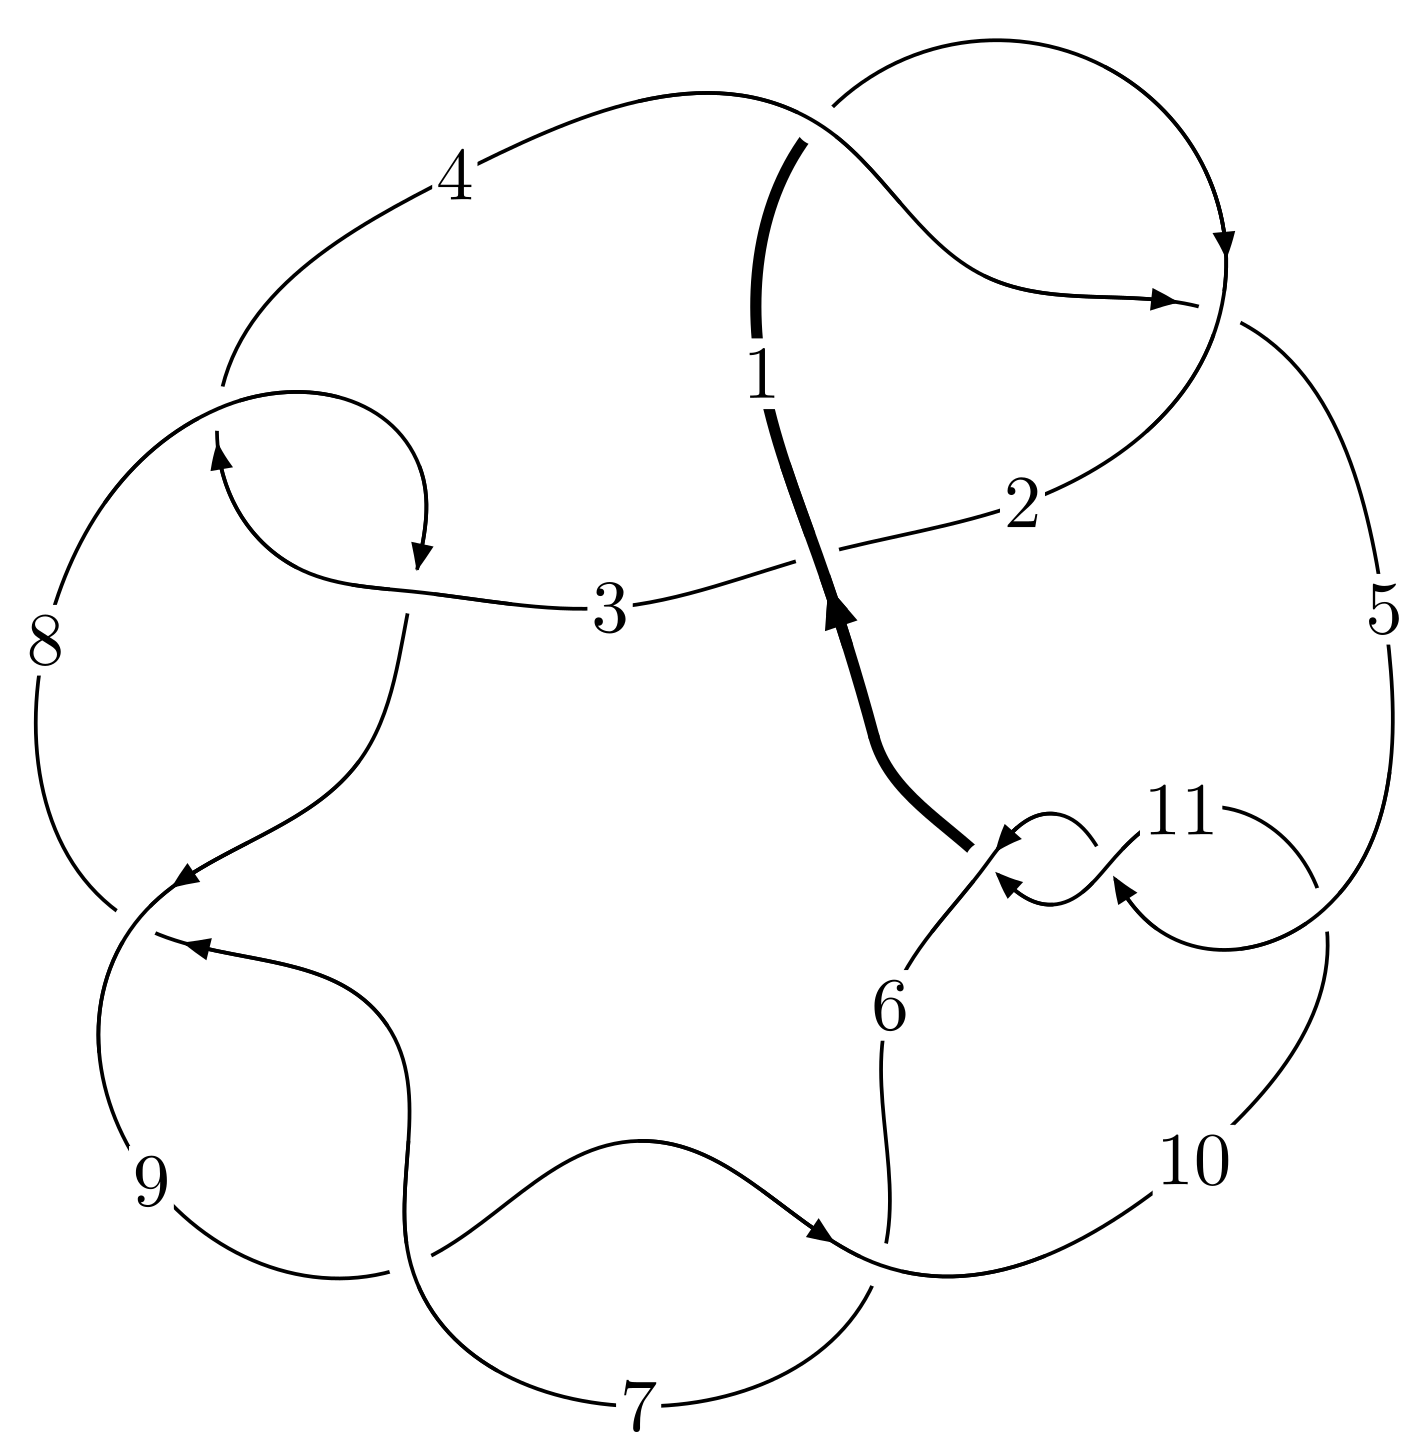
\includegraphics[width=112pt]{../../../GIT/diagram.site/Diagrams/png/307_11a_58.png}\\
\ \ \ A knot diagram\footnotemark}&
\allowdisplaybreaks
\textbf{Linearized knot diagam} \\
\cline{2-2}
 &
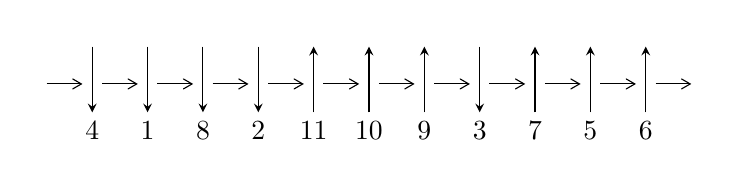
\begin{tikzpicture}[x=20pt, y=17pt]
	% nodes
	\node (C0) at (0, 0) {};
	\node (C1) at (1, 0) {};
	\node (C1U) at (1, +1) {};
	\node (C1D) at (1, -1) {4};

	\node (C2) at (2, 0) {};
	\node (C2U) at (2, +1) {};
	\node (C2D) at (2, -1) {1};

	\node (C3) at (3, 0) {};
	\node (C3U) at (3, +1) {};
	\node (C3D) at (3, -1) {8};

	\node (C4) at (4, 0) {};
	\node (C4U) at (4, +1) {};
	\node (C4D) at (4, -1) {2};

	\node (C5) at (5, 0) {};
	\node (C5U) at (5, +1) {};
	\node (C5D) at (5, -1) {11};

	\node (C6) at (6, 0) {};
	\node (C6U) at (6, +1) {};
	\node (C6D) at (6, -1) {10};

	\node (C7) at (7, 0) {};
	\node (C7U) at (7, +1) {};
	\node (C7D) at (7, -1) {9};

	\node (C8) at (8, 0) {};
	\node (C8U) at (8, +1) {};
	\node (C8D) at (8, -1) {3};

	\node (C9) at (9, 0) {};
	\node (C9U) at (9, +1) {};
	\node (C9D) at (9, -1) {7};

	\node (C10) at (10, 0) {};
	\node (C10U) at (10, +1) {};
	\node (C10D) at (10, -1) {5};

	\node (C11) at (11, 0) {};
	\node (C11U) at (11, +1) {};
	\node (C11D) at (11, -1) {6};
	\node (C12) at (12, 0) {};

	% arrows
	\draw[->,>={angle 60}]
	(C0) edge (C1) (C1) edge (C2) (C2) edge (C3) (C3) edge (C4) (C4) edge (C5) (C5) edge (C6) (C6) edge (C7) (C7) edge (C8) (C8) edge (C9) (C9) edge (C10) (C10) edge (C11) (C11) edge (C12) ;	\draw[->,>=stealth]
	(C1U) edge (C1D) (C2U) edge (C2D) (C3U) edge (C3D) (C4U) edge (C4D) (C5D) edge (C5U) (C6D) edge (C6U) (C7D) edge (C7U) (C8U) edge (C8D) (C9D) edge (C9U) (C10D) edge (C10U) (C11D) edge (C11U) ;
	\end{tikzpicture} \\
\hhline{~~} \\& 
\textbf{Solving Sequence} \\ \cline{2-2} 
 &
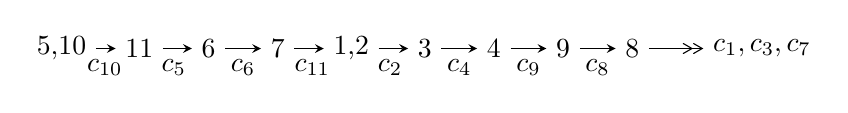
\begin{tikzpicture}[x=25pt, y=7pt]
	% node
	\node (A0) at (-1/8, 0) {5,10};
	\node (A1) at (1, 0) {11};
	\node (A2) at (2, 0) {6};
	\node (A3) at (3, 0) {7};
	\node (A4) at (65/16, 0) {1,2};
	\node (A5) at (41/8, 0) {3};
	\node (A6) at (49/8, 0) {4};
	\node (A7) at (57/8, 0) {9};
	\node (A8) at (65/8, 0) {8};
	\node (C1) at (1/2, -1) {$c_{10}$};
	\node (C2) at (3/2, -1) {$c_{5}$};
	\node (C3) at (5/2, -1) {$c_{6}$};
	\node (C4) at (7/2, -1) {$c_{11}$};
	\node (C5) at (37/8, -1) {$c_{2}$};
	\node (C6) at (45/8, -1) {$c_{4}$};
	\node (C7) at (53/8, -1) {$c_{9}$};
	\node (C8) at (61/8, -1) {$c_{8}$};
	\node (A9) at (10, 0) {$c_{1},c_{3},c_{7}$};

	% edge
	\draw[->,>=stealth]	
	(A0) edge (A1) (A1) edge (A2) (A2) edge (A3) (A3) edge (A4) (A4) edge (A5) (A5) edge (A6) (A6) edge (A7) (A7) edge (A8) ;
	\draw[->>,>={angle 60}]	
	(A8) edge (A9);
\end{tikzpicture} \\ 

\end{tabular} \\

\footnotetext{
The image of knot diagram is generated by the software ``\textbf{Draw programme}" developed by Andrew Bartholomew(\url{http://www.layer8.co.uk/maths/draw/index.htm\#Running-draw}), where we modified some parts for our purpose(\url{https://github.com/CATsTAILs/LinksPainter}).
}\phantom \\ \newline 
\centering \textbf{Ideals for irreducible components\footnotemark of $X_{\text{par}}$} 
 
\begin{align*}
I^u_{1}&=\langle 
u^{25}-9 u^{23}+\cdots+b+u,\;- u^{28}- u^{27}+\cdots+a-3,\;u^{29}+2 u^{28}+\cdots+3 u+1\rangle \\
I^u_{2}&=\langle 
u^2+b,\;a-1,\;u^{12}-4 u^{10}+u^9+6 u^8-3 u^7- u^6+3 u^5-5 u^4+u^3+3 u^2-2 u+1\rangle \\
I^u_{3}&=\langle 
b+1,\;a-1,\;u-1\rangle \\
\\
\end{align*}
\raggedright * 3 irreducible components of $\dim_{\mathbb{C}}=0$, with total 42 representations.\\
\footnotetext{All coefficients of polynomials are rational numbers. But the coefficients are sometimes approximated in decimal forms when there is not enough margin.}
\newpage
\renewcommand{\arraystretch}{1}
\centering \section*{I. $I^u_{1}= \langle u^{25}-9 u^{23}+\cdots+b+u,\;- u^{28}- u^{27}+\cdots+a-3,\;u^{29}+2 u^{28}+\cdots+3 u+1 \rangle$}
\flushleft \textbf{(i) Arc colorings}\\
\begin{tabular}{m{7pt} m{180pt} m{7pt} m{180pt} }
\flushright $a_{5}=$&$\begin{pmatrix}0\\u\end{pmatrix}$ \\
\flushright $a_{10}=$&$\begin{pmatrix}1\\0\end{pmatrix}$ \\
\flushright $a_{11}=$&$\begin{pmatrix}1\\- u^2\end{pmatrix}$ \\
\flushright $a_{6}=$&$\begin{pmatrix}u\\- u^3+u\end{pmatrix}$ \\
\flushright $a_{7}=$&$\begin{pmatrix}- u^3+2 u\\- u^3+u\end{pmatrix}$ \\
\flushright $a_{1}=$&$\begin{pmatrix}- u^2+1\\u^4-2 u^2\end{pmatrix}$ \\
\flushright $a_{2}=$&$\begin{pmatrix}u^{28}+u^{27}+\cdots-5 u+3\\- u^{25}+9 u^{23}+\cdots+4 u^2- u\end{pmatrix}$ \\
\flushright $a_{3}=$&$\begin{pmatrix}- u^{28}+11 u^{26}+\cdots-8 u+1\\u^{28}+u^{27}+\cdots+u+1\end{pmatrix}$ \\
\flushright $a_{4}=$&$\begin{pmatrix}- u^{27}+11 u^{25}+\cdots+6 u-2\\- u^{28}- u^{27}+\cdots- u-1\end{pmatrix}$ \\
\flushright $a_{9}=$&$\begin{pmatrix}u^6-3 u^4+2 u^2+1\\u^6-2 u^4+u^2\end{pmatrix}$ \\
\flushright $a_{8}=$&$\begin{pmatrix}- u^9+4 u^7-5 u^5+3 u\\- u^9+3 u^7-3 u^5+u\end{pmatrix}$\\ \flushright $a_{8}=$&$\begin{pmatrix}- u^9+4 u^7-5 u^5+3 u\\- u^9+3 u^7-3 u^5+u\end{pmatrix}$\\&\end{tabular}
\flushleft \textbf{(ii) Obstruction class $= -1$}\\~\\
\flushleft \textbf{(iii) Cusp Shapes $= -4 u^{28}-6 u^{27}+40 u^{26}+58 u^{25}-176 u^{24}-236 u^{23}+428 u^{22}+482 u^{21}-568 u^{20}-370 u^{19}+236 u^{18}-414 u^{17}+460 u^{16}+1092 u^{15}-788 u^{14}-532 u^{13}+356 u^{12}-584 u^{11}+236 u^{10}+608 u^9-308 u^8+84 u^7+40 u^6-178 u^5+60 u^4-26 u^3+8 u^2+6 u-8$}\\~\\
\newpage\renewcommand{\arraystretch}{1}
\flushleft \textbf{(iv) u-Polynomials at the component}\newline \\
\begin{tabular}{m{50pt}|m{274pt}}
Crossings & \hspace{64pt}u-Polynomials at each crossing \\
\hline $$\begin{aligned}c_{1},c_{4}\end{aligned}$$&$\begin{aligned}
&u^{29}-2 u^{28}+\cdots- u+1
\end{aligned}$\\
\hline $$\begin{aligned}c_{2}\end{aligned}$$&$\begin{aligned}
&u^{29}+16 u^{28}+\cdots+7 u+1
\end{aligned}$\\
\hline $$\begin{aligned}c_{3},c_{8}\end{aligned}$$&$\begin{aligned}
&u^{29}+2 u^{28}+\cdots+2 u+2
\end{aligned}$\\
\hline $$\begin{aligned}c_{5},c_{10},c_{11}\end{aligned}$$&$\begin{aligned}
&u^{29}+2 u^{28}+\cdots+3 u+1
\end{aligned}$\\
\hline $$\begin{aligned}c_{6},c_{7},c_{9}\end{aligned}$$&$\begin{aligned}
&u^{29}-6 u^{28}+\cdots+8 u+4
\end{aligned}$\\
\hline
\end{tabular}\\~\\
\newpage\renewcommand{\arraystretch}{1}
\flushleft \textbf{(v) Riley Polynomials at the component}\newline \\
\begin{tabular}{m{50pt}|m{274pt}}
Crossings & \hspace{64pt}Riley Polynomials at each crossing \\
\hline $$\begin{aligned}c_{1},c_{4}\end{aligned}$$&$\begin{aligned}
&y^{29}-16 y^{28}+\cdots+7 y-1
\end{aligned}$\\
\hline $$\begin{aligned}c_{2}\end{aligned}$$&$\begin{aligned}
&y^{29}-4 y^{28}+\cdots-17 y-1
\end{aligned}$\\
\hline $$\begin{aligned}c_{3},c_{8}\end{aligned}$$&$\begin{aligned}
&y^{29}+6 y^{28}+\cdots+8 y-4
\end{aligned}$\\
\hline $$\begin{aligned}c_{5},c_{10},c_{11}\end{aligned}$$&$\begin{aligned}
&y^{29}-24 y^{28}+\cdots+23 y-1
\end{aligned}$\\
\hline $$\begin{aligned}c_{6},c_{7},c_{9}\end{aligned}$$&$\begin{aligned}
&y^{29}+30 y^{28}+\cdots+504 y-16
\end{aligned}$\\
\hline
\end{tabular}\\~\\
\newpage\flushleft \textbf{(vi) Complex Volumes and Cusp Shapes}
$$\begin{array}{c|c|c}  
\text{Solutions to }I^u_{1}& \I (\text{vol} + \sqrt{-1}CS) & \text{Cusp shape}\\
 \hline 
\begin{aligned}
u &= \phantom{-}0.050913 + 0.910185 I \\
a &= -0.45193 - 1.39576 I \\
b &= \phantom{-}0.00992 - 2.35228 I\end{aligned}
 & -10.46170 + 8.03356 I & -4.76249 - 5.59744 I \\ \hline\begin{aligned}
u &= \phantom{-}0.050913 - 0.910185 I \\
a &= -0.45193 + 1.39576 I \\
b &= \phantom{-}0.00992 + 2.35228 I\end{aligned}
 & -10.46170 - 8.03356 I & -4.76249 + 5.59744 I \\ \hline\begin{aligned}
u &= -0.008721 + 0.887960 I \\
a &= -0.49123 + 1.42056 I \\
b &= \phantom{-}0.14380 + 2.36020 I\end{aligned}
 & -10.71030 - 1.52343 I & -5.35413 + 0.68771 I \\ \hline\begin{aligned}
u &= -0.008721 - 0.887960 I \\
a &= -0.49123 - 1.42056 I \\
b &= \phantom{-}0.14380 - 2.36020 I\end{aligned}
 & -10.71030 + 1.52343 I & -5.35413 - 0.68771 I \\ \hline\begin{aligned}
u &= \phantom{-}1.189730 + 0.056062 I \\
a &= -0.370086 - 0.255115 I \\
b &= -1.23899 - 0.69502 I\end{aligned}
 & \phantom{-}2.39907 + 0.12369 I & \phantom{-}3.50407 + 1.07759 I \\ \hline\begin{aligned}
u &= \phantom{-}1.189730 - 0.056062 I \\
a &= -0.370086 + 0.255115 I \\
b &= -1.23899 + 0.69502 I\end{aligned}
 & \phantom{-}2.39907 - 0.12369 I & \phantom{-}3.50407 - 1.07759 I \\ \hline\begin{aligned}
u &= \phantom{-}1.242320 + 0.189774 I \\
a &= -0.715591 + 0.438399 I \\
b &= \phantom{-}0.20240 + 2.88734 I\end{aligned}
 & \phantom{-}0.91595 + 3.56420 I & \phantom{-}0.67873 - 4.99863 I \\ \hline\begin{aligned}
u &= \phantom{-}1.242320 - 0.189774 I \\
a &= -0.715591 - 0.438399 I \\
b &= \phantom{-}0.20240 - 2.88734 I\end{aligned}
 & \phantom{-}0.91595 - 3.56420 I & \phantom{-}0.67873 + 4.99863 I \\ \hline\begin{aligned}
u &= \phantom{-}0.230236 + 0.672244 I \\
a &= -0.11327 - 1.56979 I \\
b &= -0.07670 - 1.55700 I\end{aligned}
 & -1.85869 + 5.19499 I & -2.04173 - 8.30480 I \\ \hline\begin{aligned}
u &= \phantom{-}0.230236 - 0.672244 I \\
a &= -0.11327 + 1.56979 I \\
b &= -0.07670 + 1.55700 I\end{aligned}
 & -1.85869 - 5.19499 I & -2.04173 + 8.30480 I\\
 \hline 
 \end{array}$$\newpage$$\begin{array}{c|c|c}  
\text{Solutions to }I^u_{1}& \I (\text{vol} + \sqrt{-1}CS) & \text{Cusp shape}\\
 \hline 
\begin{aligned}
u &= \phantom{-}1.249690 + 0.417811 I \\
a &= -0.215564 - 0.608911 I \\
b &= -0.927812 - 0.165212 I\end{aligned}
 & -3.02235 + 1.47420 I & \phantom{-}1.47993 - 0.60903 I \\ \hline\begin{aligned}
u &= \phantom{-}1.249690 - 0.417811 I \\
a &= -0.215564 + 0.608911 I \\
b &= -0.927812 + 0.165212 I\end{aligned}
 & -3.02235 - 1.47420 I & \phantom{-}1.47993 + 0.60903 I \\ \hline\begin{aligned}
u &= -1.311940 + 0.179476 I \\
a &= -0.339083 + 0.475947 I \\
b &= -0.644137 + 0.471467 I\end{aligned}
 & \phantom{-}4.98921 - 3.78682 I & \phantom{-}7.27007 + 4.16727 I \\ \hline\begin{aligned}
u &= -1.311940 - 0.179476 I \\
a &= -0.339083 - 0.475947 I \\
b &= -0.644137 - 0.471467 I\end{aligned}
 & \phantom{-}4.98921 + 3.78682 I & \phantom{-}7.27007 - 4.16727 I \\ \hline\begin{aligned}
u &= -1.342150 + 0.040293 I \\
a &= -0.537408 - 0.444706 I \\
b &= -0.23164 - 1.41782 I\end{aligned}
 & \phantom{-}6.61715 - 2.27209 I & \phantom{-}8.89752 + 3.80982 I \\ \hline\begin{aligned}
u &= -1.342150 - 0.040293 I \\
a &= -0.537408 + 0.444706 I \\
b &= -0.23164 + 1.41782 I\end{aligned}
 & \phantom{-}6.61715 + 2.27209 I & \phantom{-}8.89752 - 3.80982 I \\ \hline\begin{aligned}
u &= \phantom{-}1.286000 + 0.418935 I \\
a &= -0.762208 + 0.613998 I \\
b &= \phantom{-}1.69138 + 2.74611 I\end{aligned}
 & -6.68464 + 6.20004 I & -1.73580 - 3.81481 I \\ \hline\begin{aligned}
u &= \phantom{-}1.286000 - 0.418935 I \\
a &= -0.762208 - 0.613998 I \\
b &= \phantom{-}1.69138 - 2.74611 I\end{aligned}
 & -6.68464 - 6.20004 I & -1.73580 + 3.81481 I \\ \hline\begin{aligned}
u &= -1.333980 + 0.244603 I \\
a &= -0.683762 - 0.524847 I \\
b &= \phantom{-}0.83387 - 2.33932 I\end{aligned}
 & \phantom{-}3.04589 - 8.42692 I & \phantom{-}3.52830 + 8.66921 I \\ \hline\begin{aligned}
u &= -1.333980 - 0.244603 I \\
a &= -0.683762 + 0.524847 I \\
b &= \phantom{-}0.83387 + 2.33932 I\end{aligned}
 & \phantom{-}3.04589 + 8.42692 I & \phantom{-}3.52830 - 8.66921 I\\
 \hline 
 \end{array}$$\newpage$$\begin{array}{c|c|c}  
\text{Solutions to }I^u_{1}& \I (\text{vol} + \sqrt{-1}CS) & \text{Cusp shape}\\
 \hline 
\begin{aligned}
u &= -1.301320 + 0.407588 I \\
a &= -0.248387 + 0.609615 I \\
b &= -0.872384 + 0.107277 I\end{aligned}
 & -2.63518 - 7.77071 I & \phantom{-}2.10858 + 5.30383 I \\ \hline\begin{aligned}
u &= -1.301320 - 0.407588 I \\
a &= -0.248387 - 0.609615 I \\
b &= -0.872384 - 0.107277 I\end{aligned}
 & -2.63518 + 7.77071 I & \phantom{-}2.10858 - 5.30383 I \\ \hline\begin{aligned}
u &= \phantom{-}0.529946 + 0.329108 I \\
a &= \phantom{-}0.667313 - 0.986592 I \\
b &= -0.347726 - 0.588274 I\end{aligned}
 & \phantom{-}0.93542 + 1.41053 I & \phantom{-}5.39446 - 5.74020 I \\ \hline\begin{aligned}
u &= \phantom{-}0.529946 - 0.329108 I \\
a &= \phantom{-}0.667313 + 0.986592 I \\
b &= -0.347726 + 0.588274 I\end{aligned}
 & \phantom{-}0.93542 - 1.41053 I & \phantom{-}5.39446 + 5.74020 I \\ \hline\begin{aligned}
u &= -1.320520 + 0.424615 I \\
a &= -0.743481 - 0.622059 I \\
b &= \phantom{-}1.72687 - 2.60904 I\end{aligned}
 & -6.1783 - 12.8069 I & -0.92308 + 8.12569 I \\ \hline\begin{aligned}
u &= -1.320520 - 0.424615 I \\
a &= -0.743481 + 0.622059 I \\
b &= \phantom{-}1.72687 + 2.60904 I\end{aligned}
 & -6.1783 + 12.8069 I & -0.92308 - 8.12569 I \\ \hline\begin{aligned}
u &= -0.063245 + 0.516212 I \\
a &= -0.28684 + 2.09363 I \\
b &= \phantom{-}0.49644 + 1.38676 I\end{aligned}
 & -3.02142 - 1.01433 I & -6.77496 + 0.83339 I \\ \hline\begin{aligned}
u &= -0.063245 - 0.516212 I \\
a &= -0.28684 - 2.09363 I \\
b &= \phantom{-}0.49644 - 1.38676 I\end{aligned}
 & -3.02142 + 1.01433 I & -6.77496 - 0.83339 I \\ \hline\begin{aligned}
u &= -0.193938\phantom{ +0.000000I} \\
a &= \phantom{-}4.58305\phantom{ +0.000000I} \\
b &= \phantom{-}0.469396\phantom{ +0.000000I}\end{aligned}
 & -1.29813\phantom{ +0.000000I} & -8.53890\phantom{ +0.000000I}\\
 \hline 
 \end{array}$$\newpage\newpage\renewcommand{\arraystretch}{1}
\centering \section*{II. $I^u_{2}= \langle u^2+b,\;a-1,\;u^{12}-4 u^{10}+\cdots-2 u+1 \rangle$}
\flushleft \textbf{(i) Arc colorings}\\
\begin{tabular}{m{7pt} m{180pt} m{7pt} m{180pt} }
\flushright $a_{5}=$&$\begin{pmatrix}0\\u\end{pmatrix}$ \\
\flushright $a_{10}=$&$\begin{pmatrix}1\\0\end{pmatrix}$ \\
\flushright $a_{11}=$&$\begin{pmatrix}1\\- u^2\end{pmatrix}$ \\
\flushright $a_{6}=$&$\begin{pmatrix}u\\- u^3+u\end{pmatrix}$ \\
\flushright $a_{7}=$&$\begin{pmatrix}- u^3+2 u\\- u^3+u\end{pmatrix}$ \\
\flushright $a_{1}=$&$\begin{pmatrix}- u^2+1\\u^4-2 u^2\end{pmatrix}$ \\
\flushright $a_{2}=$&$\begin{pmatrix}1\\- u^2\end{pmatrix}$ \\
\flushright $a_{3}=$&$\begin{pmatrix}u^4- u^2+1\\- u^6+2 u^4- u^2\end{pmatrix}$ \\
\flushright $a_{4}=$&$\begin{pmatrix}u\\- u^3+u\end{pmatrix}$ \\
\flushright $a_{9}=$&$\begin{pmatrix}u^6-3 u^4+2 u^2+1\\u^6-2 u^4+u^2\end{pmatrix}$ \\
\flushright $a_{8}=$&$\begin{pmatrix}- u^9+4 u^7-5 u^5+3 u\\- u^9+3 u^7-3 u^5+u\end{pmatrix}$\\ \flushright $a_{8}=$&$\begin{pmatrix}- u^9+4 u^7-5 u^5+3 u\\- u^9+3 u^7-3 u^5+u\end{pmatrix}$\\&\end{tabular}
\flushleft \textbf{(ii) Obstruction class $= -1$}\\~\\
\flushleft \textbf{(iii) Cusp Shapes $= 4 u^9-12 u^7+4 u^6+12 u^5-8 u^4+8 u^3+4 u^2-12 u+6$}\\~\\
\newpage\renewcommand{\arraystretch}{1}
\flushleft \textbf{(iv) u-Polynomials at the component}\newline \\
\begin{tabular}{m{50pt}|m{274pt}}
Crossings & \hspace{64pt}u-Polynomials at each crossing \\
\hline $$\begin{aligned}c_{1},c_{4},c_{5}\\c_{10},c_{11}\end{aligned}$$&$\begin{aligned}
&u^{12}-4 u^{10}+u^9+6 u^8-3 u^7- u^6+3 u^5-5 u^4+u^3+3 u^2-2 u+1
\end{aligned}$\\
\hline $$\begin{aligned}c_{2}\end{aligned}$$&$\begin{aligned}
&u^{12}+8 u^{11}+\cdots-2 u+1
\end{aligned}$\\
\hline $$\begin{aligned}c_{3},c_{8}\end{aligned}$$&$\begin{aligned}
&(u^4- u^3+u^2+1)^3
\end{aligned}$\\
\hline $$\begin{aligned}c_{6},c_{7},c_{9}\end{aligned}$$&$\begin{aligned}
&(u^4- u^3+3 u^2-2 u+1)^3
\end{aligned}$\\
\hline
\end{tabular}\\~\\
\newpage\renewcommand{\arraystretch}{1}
\flushleft \textbf{(v) Riley Polynomials at the component}\newline \\
\begin{tabular}{m{50pt}|m{274pt}}
Crossings & \hspace{64pt}Riley Polynomials at each crossing \\
\hline $$\begin{aligned}c_{1},c_{4},c_{5}\\c_{10},c_{11}\end{aligned}$$&$\begin{aligned}
&y^{12}-8 y^{11}+\cdots+2 y+1
\end{aligned}$\\
\hline $$\begin{aligned}c_{2}\end{aligned}$$&$\begin{aligned}
&y^{12}-8 y^{11}+\cdots+2 y+1
\end{aligned}$\\
\hline $$\begin{aligned}c_{3},c_{8}\end{aligned}$$&$\begin{aligned}
&(y^4+y^3+3 y^2+2 y+1)^3
\end{aligned}$\\
\hline $$\begin{aligned}c_{6},c_{7},c_{9}\end{aligned}$$&$\begin{aligned}
&(y^4+5 y^3+7 y^2+2 y+1)^3
\end{aligned}$\\
\hline
\end{tabular}\\~\\
\newpage\flushleft \textbf{(vi) Complex Volumes and Cusp Shapes}
$$\begin{array}{c|c|c}  
\text{Solutions to }I^u_{2}& \I (\text{vol} + \sqrt{-1}CS) & \text{Cusp shape}\\
 \hline 
\begin{aligned}
u &= \phantom{-}0.944825 + 0.321917 I \\
a &= \phantom{-}1.00000\phantom{ +0.000000I} \\
b &= -0.789064 - 0.608311 I\end{aligned}
 & \phantom{-}0.21101 - 1.41510 I & \phantom{-}1.82674 + 4.90874 I \\ \hline\begin{aligned}
u &= \phantom{-}0.944825 - 0.321917 I \\
a &= \phantom{-}1.00000\phantom{ +0.000000I} \\
b &= -0.789064 + 0.608311 I\end{aligned}
 & \phantom{-}0.21101 + 1.41510 I & \phantom{-}1.82674 - 4.90874 I \\ \hline\begin{aligned}
u &= \phantom{-}0.031664 + 0.878090 I \\
a &= \phantom{-}1.00000\phantom{ +0.000000I} \\
b &= \phantom{-}0.770039 - 0.055609 I\end{aligned}
 & -6.79074 + 3.16396 I & -1.82674 - 2.56480 I \\ \hline\begin{aligned}
u &= \phantom{-}0.031664 - 0.878090 I \\
a &= \phantom{-}1.00000\phantom{ +0.000000I} \\
b &= \phantom{-}0.770039 + 0.055609 I\end{aligned}
 & -6.79074 - 3.16396 I & -1.82674 + 2.56480 I \\ \hline\begin{aligned}
u &= -1.186690 + 0.158407 I \\
a &= \phantom{-}1.00000\phantom{ +0.000000I} \\
b &= -1.38315 + 0.37596 I\end{aligned}
 & \phantom{-}0.21101 - 1.41510 I & \phantom{-}1.82674 + 4.90874 I \\ \hline\begin{aligned}
u &= -1.186690 - 0.158407 I \\
a &= \phantom{-}1.00000\phantom{ +0.000000I} \\
b &= -1.38315 - 0.37596 I\end{aligned}
 & \phantom{-}0.21101 + 1.41510 I & \phantom{-}1.82674 - 4.90874 I \\ \hline\begin{aligned}
u &= \phantom{-}1.240280 + 0.455646 I \\
a &= \phantom{-}1.00000\phantom{ +0.000000I} \\
b &= -1.33067 - 1.13025 I\end{aligned}
 & -6.79074 - 3.16396 I & -1.82674 + 2.56480 I \\ \hline\begin{aligned}
u &= \phantom{-}1.240280 - 0.455646 I \\
a &= \phantom{-}1.00000\phantom{ +0.000000I} \\
b &= -1.33067 + 1.13025 I\end{aligned}
 & -6.79074 + 3.16396 I & -1.82674 - 2.56480 I \\ \hline\begin{aligned}
u &= -1.271940 + 0.422443 I \\
a &= \phantom{-}1.00000\phantom{ +0.000000I} \\
b &= -1.43937 + 1.07464 I\end{aligned}
 & -6.79074 - 3.16396 I & -1.82674 + 2.56480 I \\ \hline\begin{aligned}
u &= -1.271940 - 0.422443 I \\
a &= \phantom{-}1.00000\phantom{ +0.000000I} \\
b &= -1.43937 - 1.07464 I\end{aligned}
 & -6.79074 + 3.16396 I & -1.82674 - 2.56480 I\\
 \hline 
 \end{array}$$\newpage$$\begin{array}{c|c|c}  
\text{Solutions to }I^u_{2}& \I (\text{vol} + \sqrt{-1}CS) & \text{Cusp shape}\\
 \hline 
\begin{aligned}
u &= \phantom{-}0.241868 + 0.480324 I \\
a &= \phantom{-}1.00000\phantom{ +0.000000I} \\
b &= \phantom{-}0.172212 - 0.232350 I\end{aligned}
 & \phantom{-}0.21101 + 1.41510 I & \phantom{-}1.82674 - 4.90874 I \\ \hline\begin{aligned}
u &= \phantom{-}0.241868 - 0.480324 I \\
a &= \phantom{-}1.00000\phantom{ +0.000000I} \\
b &= \phantom{-}0.172212 + 0.232350 I\end{aligned}
 & \phantom{-}0.21101 - 1.41510 I & \phantom{-}1.82674 + 4.90874 I\\
 \hline 
 \end{array}$$\newpage\newpage\renewcommand{\arraystretch}{1}
\centering \section*{III. $I^u_{3}= \langle b+1,\;a-1,\;u-1 \rangle$}
\flushleft \textbf{(i) Arc colorings}\\
\begin{tabular}{m{7pt} m{180pt} m{7pt} m{180pt} }
\flushright $a_{5}=$&$\begin{pmatrix}0\\1\end{pmatrix}$ \\
\flushright $a_{10}=$&$\begin{pmatrix}1\\0\end{pmatrix}$ \\
\flushright $a_{11}=$&$\begin{pmatrix}1\\-1\end{pmatrix}$ \\
\flushright $a_{6}=$&$\begin{pmatrix}1\\0\end{pmatrix}$ \\
\flushright $a_{7}=$&$\begin{pmatrix}1\\0\end{pmatrix}$ \\
\flushright $a_{1}=$&$\begin{pmatrix}0\\-1\end{pmatrix}$ \\
\flushright $a_{2}=$&$\begin{pmatrix}1\\-1\end{pmatrix}$ \\
\flushright $a_{3}=$&$\begin{pmatrix}1\\0\end{pmatrix}$ \\
\flushright $a_{4}=$&$\begin{pmatrix}1\\0\end{pmatrix}$ \\
\flushright $a_{9}=$&$\begin{pmatrix}1\\0\end{pmatrix}$ \\
\flushright $a_{8}=$&$\begin{pmatrix}1\\0\end{pmatrix}$\\ \flushright $a_{8}=$&$\begin{pmatrix}1\\0\end{pmatrix}$\\&\end{tabular}
\flushleft \textbf{(ii) Obstruction class $= 1$}\\~\\
\flushleft \textbf{(iii) Cusp Shapes $= 0$}\\~\\
\newpage\renewcommand{\arraystretch}{1}
\flushleft \textbf{(iv) u-Polynomials at the component}\newline \\
\begin{tabular}{m{50pt}|m{274pt}}
Crossings & \hspace{64pt}u-Polynomials at each crossing \\
\hline $$\begin{aligned}c_{1},c_{10},c_{11}\end{aligned}$$&$\begin{aligned}
&u-1
\end{aligned}$\\
\hline $$\begin{aligned}c_{2},c_{4},c_{5}\end{aligned}$$&$\begin{aligned}
&u+1
\end{aligned}$\\
\hline $$\begin{aligned}c_{3},c_{6},c_{7}\\c_{8},c_{9}\end{aligned}$$&$\begin{aligned}
&u
\end{aligned}$\\
\hline
\end{tabular}\\~\\
\newpage\renewcommand{\arraystretch}{1}
\flushleft \textbf{(v) Riley Polynomials at the component}\newline \\
\begin{tabular}{m{50pt}|m{274pt}}
Crossings & \hspace{64pt}Riley Polynomials at each crossing \\
\hline $$\begin{aligned}c_{1},c_{2},c_{4}\\c_{5},c_{10},c_{11}\end{aligned}$$&$\begin{aligned}
&y-1
\end{aligned}$\\
\hline $$\begin{aligned}c_{3},c_{6},c_{7}\\c_{8},c_{9}\end{aligned}$$&$\begin{aligned}
&y
\end{aligned}$\\
\hline
\end{tabular}\\~\\
\newpage\flushleft \textbf{(vi) Complex Volumes and Cusp Shapes}
$$\begin{array}{c|c|c}  
\text{Solutions to }I^u_{3}& \I (\text{vol} + \sqrt{-1}CS) & \text{Cusp shape}\\
 \hline 
\begin{aligned}
u &= \phantom{-}1.00000\phantom{ +0.000000I} \\
a &= \phantom{-}1.00000\phantom{ +0.000000I} \\
b &= -1.00000\phantom{ +0.000000I}\end{aligned}
 & \phantom{-0.000000 } 0 & \phantom{-0.000000 } 0\\
 \hline 
 \end{array}$$\newpage
\newpage\renewcommand{\arraystretch}{1}
\centering \section*{ IV. u-Polynomials}
\begin{tabular}{m{50pt}|m{274pt}}
Crossings & \hspace{64pt}u-Polynomials at each crossing \\
\hline $$\begin{aligned}c_{1}\end{aligned}$$&$\begin{aligned}
&(u-1)(u^{12}-4 u^{10}+\cdots-2 u+1)\\
&\cdot(u^{29}-2 u^{28}+\cdots- u+1)
\end{aligned}$\\
\hline $$\begin{aligned}c_{2}\end{aligned}$$&$\begin{aligned}
&(u+1)(u^{12}+8 u^{11}+\cdots-2 u+1)(u^{29}+16 u^{28}+\cdots+7 u+1)
\end{aligned}$\\
\hline $$\begin{aligned}c_{3},c_{8}\end{aligned}$$&$\begin{aligned}
&u(u^4- u^3+u^2+1)^3(u^{29}+2 u^{28}+\cdots+2 u+2)
\end{aligned}$\\
\hline $$\begin{aligned}c_{4}\end{aligned}$$&$\begin{aligned}
&(u+1)(u^{12}-4 u^{10}+\cdots-2 u+1)\\
&\cdot(u^{29}-2 u^{28}+\cdots- u+1)
\end{aligned}$\\
\hline $$\begin{aligned}c_{5}\end{aligned}$$&$\begin{aligned}
&(u+1)(u^{12}-4 u^{10}+\cdots-2 u+1)\\
&\cdot(u^{29}+2 u^{28}+\cdots+3 u+1)
\end{aligned}$\\
\hline $$\begin{aligned}c_{6},c_{7},c_{9}\end{aligned}$$&$\begin{aligned}
&u(u^4- u^3+3 u^2-2 u+1)^{3}(u^{29}-6 u^{28}+\cdots+8 u+4)
\end{aligned}$\\
\hline $$\begin{aligned}c_{10},c_{11}\end{aligned}$$&$\begin{aligned}
&(u-1)(u^{12}-4 u^{10}+\cdots-2 u+1)\\
&\cdot(u^{29}+2 u^{28}+\cdots+3 u+1)
\end{aligned}$\\
\hline
\end{tabular}\newpage\renewcommand{\arraystretch}{1}
\centering \section*{ V. Riley Polynomials}
\begin{tabular}{m{50pt}|m{274pt}}
Crossings & \hspace{64pt}Riley Polynomials at each crossing \\
\hline $$\begin{aligned}c_{1},c_{4}\end{aligned}$$&$\begin{aligned}
&(y-1)(y^{12}-8 y^{11}+\cdots+2 y+1)(y^{29}-16 y^{28}+\cdots+7 y-1)
\end{aligned}$\\
\hline $$\begin{aligned}c_{2}\end{aligned}$$&$\begin{aligned}
&(y-1)(y^{12}-8 y^{11}+\cdots+2 y+1)(y^{29}-4 y^{28}+\cdots-17 y-1)
\end{aligned}$\\
\hline $$\begin{aligned}c_{3},c_{8}\end{aligned}$$&$\begin{aligned}
&y(y^4+y^3+3 y^2+2 y+1)^{3}(y^{29}+6 y^{28}+\cdots+8 y-4)
\end{aligned}$\\
\hline $$\begin{aligned}c_{5},c_{10},c_{11}\end{aligned}$$&$\begin{aligned}
&(y-1)(y^{12}-8 y^{11}+\cdots+2 y+1)(y^{29}-24 y^{28}+\cdots+23 y-1)
\end{aligned}$\\
\hline $$\begin{aligned}c_{6},c_{7},c_{9}\end{aligned}$$&$\begin{aligned}
&y(y^4+5 y^3+\cdots+2 y+1)^{3}(y^{29}+30 y^{28}+\cdots+504 y-16)
\end{aligned}$\\
\hline
\end{tabular}
\vskip 2pc
\end{document}